%\section{Coupling by location shifting}
%coupling_shifting
As a 3D model the waveguide can be shifted on transverse (Fig. \ref{fig:shift_x_axis} and Fig. \ref{fig:shift_y_axis}) or longitude (Fig. \ref{fig:shift_z_axis}) directions.
\begin{itemize}
\item Shift the waveguide along X-Axis: Relocate the waveguide from $-0.5\mu$m to $0.5\mu$m:
\begin{figure}[!ht]
\centering
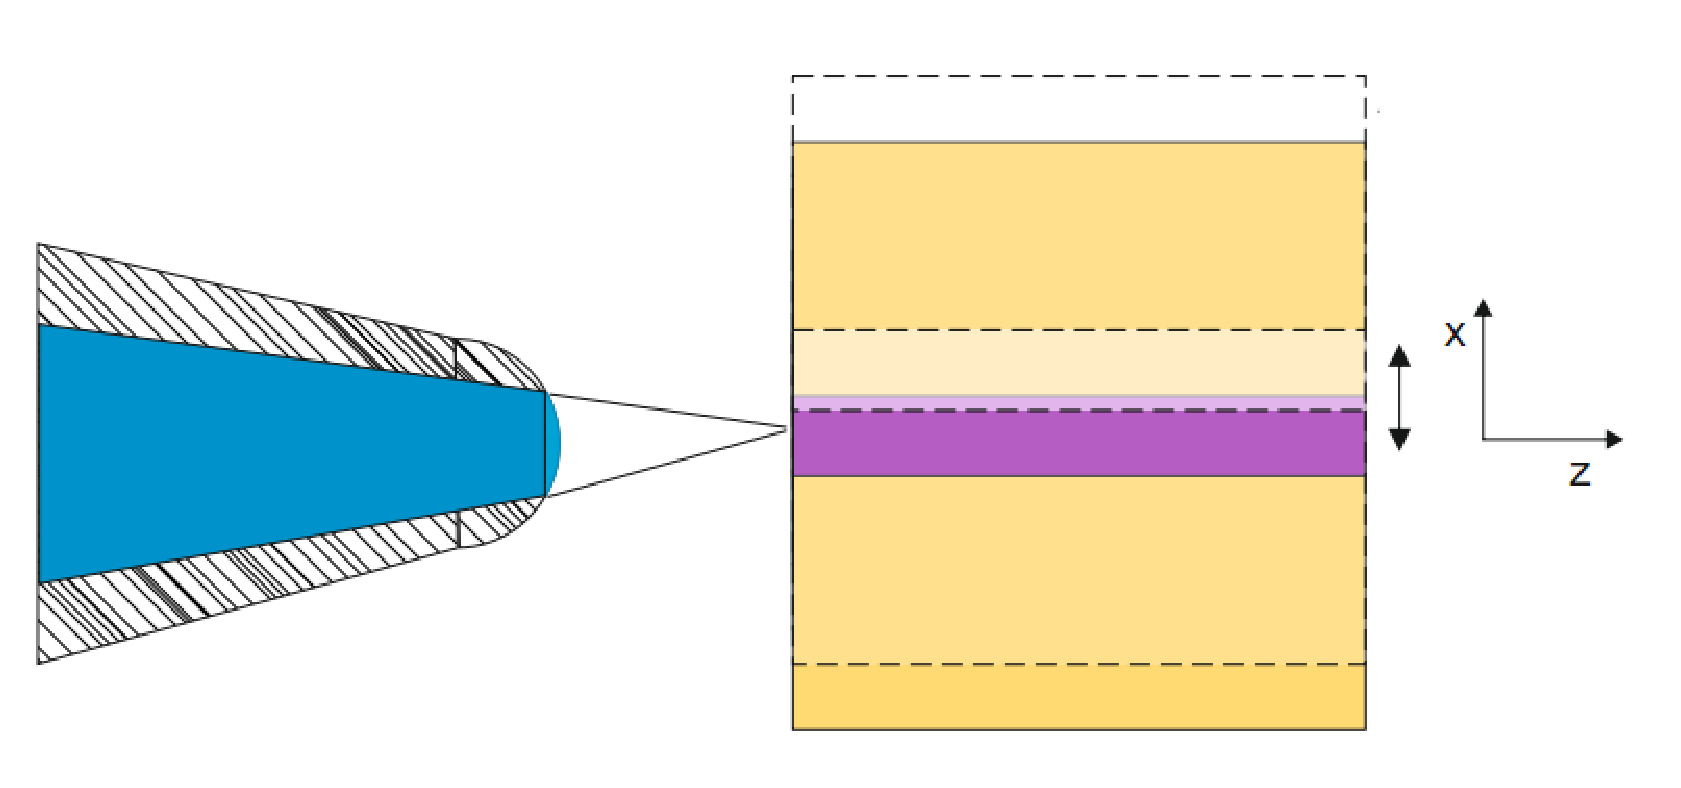
\includegraphics[width=0.7\textwidth]{bilder/shift_x_axis}
\caption{Displacing the waveguide along x-axis.}
\label{fig:shift_x_axis}
\end{figure}
\item Shift the waveguide along Y-Axis: Relocate the waveguide from $-0.5\mu$m to $0.5\mu$m:
\begin{figure}[!ht]
\centering
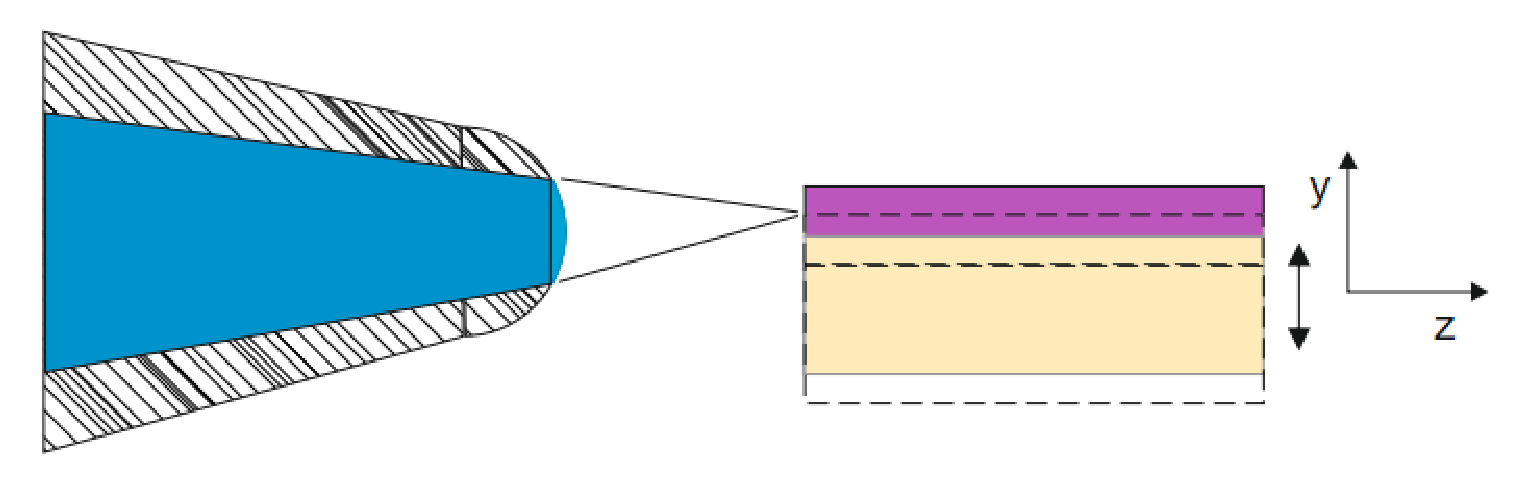
\includegraphics[width=0.7\textwidth]{bilder/shift_y_axis}
\caption{Displacing the waveguide along y-axis.}
\label{fig:shift_y_axis}
\end{figure}
\item Shift the waveguide along Z-Axis: Relocate the waveguide from $-0.5\mu$m to $0.5\mu$m:
\begin{figure}[!ht]
\centering
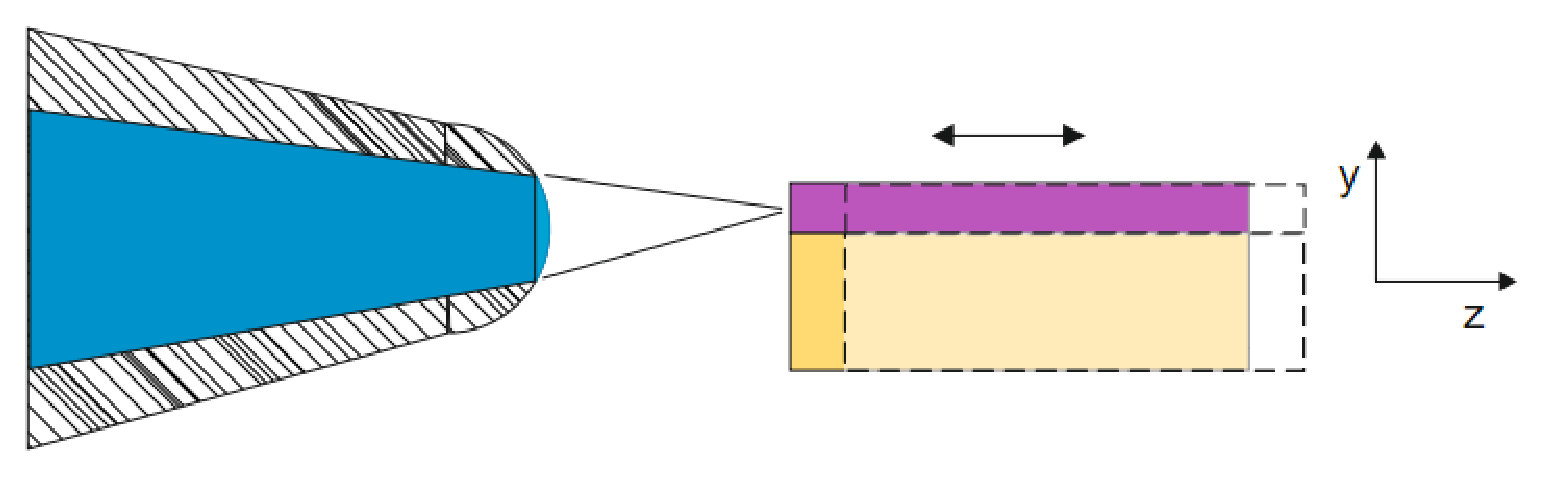
\includegraphics[width=0.7\textwidth]{bilder/shift_z_axis}
\caption{Displacing the waveguide along z-axis.}
\label{fig:shift_z_axis}
\end{figure}
\end{itemize}
Performe above arrangements and record their simulation results $|S_{21}|$ in Tab. \ref{tab:shift_result}:\\

\begin{table}[!ht]
\caption{Coupling efficiency by shifting the waveguide along X,Y and Z-Axis.}
\centering
\begin{tabular}{c|ccc}
\hline
Shift distance & X-Asis & Y-Axis & Z-Axis \\
\hline
$-0.5\mu$m 		&$32.4\%$	&$32.4\%$&$46.6\%$	\\
$-0.4\mu$m		&$37.3\%$	&$36.5\%$&$47\%$	\\
$-0.3\mu$m 		&$41.9\%$	&$41.3\%$&$48.2\%$	\\
$-0.2\mu$m	  &$45.5\%$	&$45.2\%$&$49.1\%$	\\
$-0.1\mu$m		&$48\%$	&$47.8\%$&$49.1\%$	\\
$0\mu$m			  &$48.9\%$	&$48.9\%$&$48.9\%$	\\
$0.1\mu$m			&$47.8\%$	&$48.4\%$&$48.9\%$	\\
$0.2\mu$m			&$45.5\%$	&$46.4\%$&$49.4\%$	\\
$0.3\mu$m			&$41.9\%$	&$42.9\%$&$49.7\%$	\\
$0.4\mu$m			&$37.5\%$	&$38.5\%$&$49.5\%$	\\
$0.5\mu$m			&$32.3\%$	&$33.1\%$&$48.8\%$	\\
\hline
\end{tabular}
\label{tab:shift_result}
\end{table}
\begin{figure}[!ht]
\centering
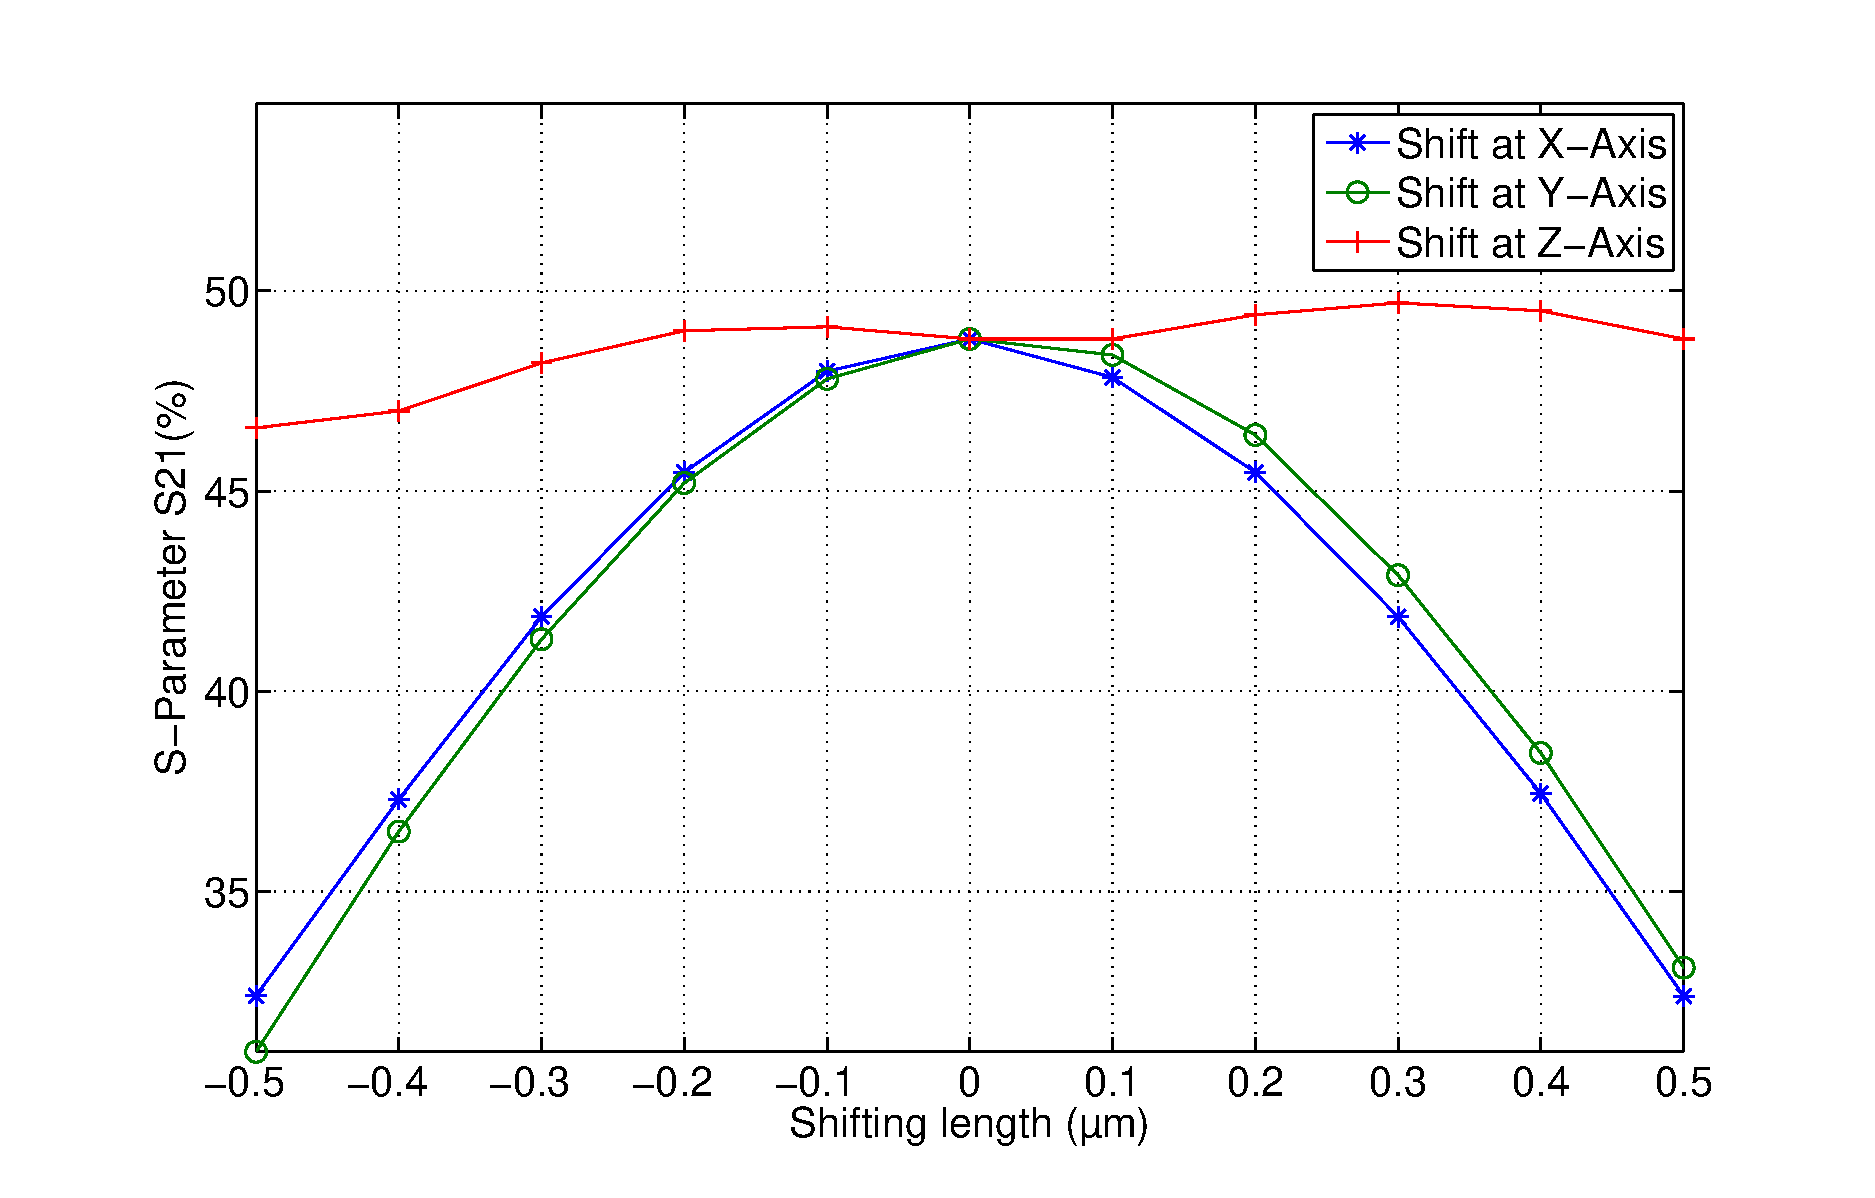
\includegraphics[width=0.8\textwidth]{bilder/shift_curve}
\caption{Coupling efficiency due to the displacement of the wavguide.}
\label{fig:shift_curve}
\end{figure}
According results in the table we can draw curves in Fig. \ref{fig:shift_curve}, which present us their coupling efficiency behavior. It is obvious that the coupling efficiency falls very quickly for vertical or horizontal shifting, while it stays relative stable for longitude displacement. From this Figure we can also reveal that coupling efficiencies are symmetric due to positive and negative X-Axis shifting. While the coupling efficiencies due to negative and positive Y-Axis shifting are not symmetric. This trend can be explained by the geometric characters of the waveguide, which is same in X-Dimension and different in Y-Dimension. And the highest coupling efficiency due to shifting along Z-Axis stands not at working distance $4\mu$m but $4.3\mu$m, which agree with the estimation of minimum spot location about $4.26\mu$m at section \ref{sect:model_model_model_TLF}. Although the minimum spot location lies not on the working distance $4\mu$m, displacement of the waveguide cannot obviously improve the coupling efficiency. Hereby the working distance will be maintained in following simulations.\\
  
